\documentclass[svgnames,table]{standalone}
%\usetheme{Madrid}
%
%
%\usepackage{animate}
%\usepackage[pdftex,active,tightpage]{preview}
\usepackage{tikz}
\usetikzlibrary{shapes,arrows,automata, positioning}
\usetikzlibrary{arrows.meta,automata,positioning}
\usepackage{float}
%\usepackage{mathpazo}

\newcounter{row}
\newcounter{col}
\newcommand\setrow[4]{
  \setcounter{col}{1}
  \foreach \n in {#1, #2, #3, #4} {
    \edef\x{\value{col} - 0.5}
    \edef\y{4.5 - \value{row}}
    \node[anchor=center] at (\x, \y) {\n};
    \stepcounter{col}
  }
  \stepcounter{row}
}



\begin{document}


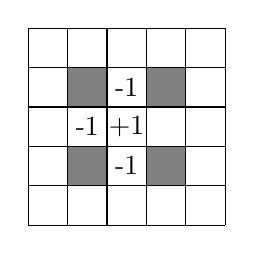
\begin{tikzpicture}
[every node/.style={minimum size=.5cm-\pgflinewidth, outer sep=0pt},
scale=.5]

  \begin{scope}
    \draw[step=1cm,color=black] (0, 0) grid (5, 5);
    %\draw[very thick, scale=3] (0, 0) grid (3, 3);

    \setcounter{row}{1}
    \setrow {}{}{-1}{}{}
    \setrow {}{-1}{+1}{}{}
    \setrow {}{}{-1}{}{}
    \setrow {}{}{}{}{}
    \node[fill=black!50] at (1.5,1.5) {};
    \node[fill=black!50] at (3.5,3.5) {};
     \node[fill=black!50] at (1.5,3.5) {};
      \node[fill=black!50] at (3.5,1.5) {};
    
    %\node[anchor=center] at (2, -1) {Maze Problem};
  \end{scope}
  
    
\end{tikzpicture}

%\end{frame}
\end{document}